\chapter[EXEMPLO DE USO]{EXEMPLO DE USO}
\label{chapter:example}

Como forma de ilustração do uso do serviço que desenvolvemos, elaboramos uma
aplicação chamada
Forensic\footnote{\url{https://gitlab.com/DGuedes/forensic}}, que interage
com o Shock via Kafka, respeitando os padrões utilizados pela API. A aplicação
foi feita em Elixir, uma linguagem funcional que utiliza a máquina virtual do
Erlang, utilizando o \textit{framework} Phoenix, que facilita no desenvolvimento
de aplicações Web.

\begin{figure}[hbt]
  \centering
  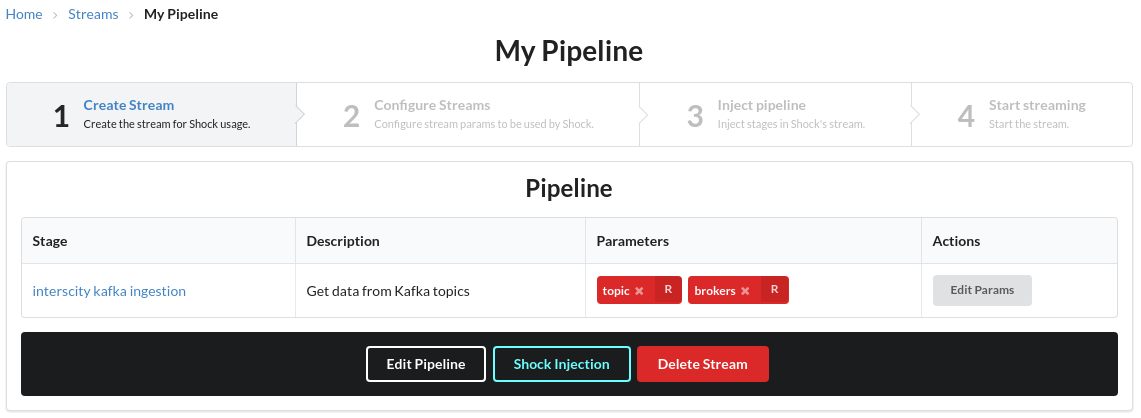
\includegraphics[width=\textwidth]{figuras/pipeline.png}
    \caption{Página de configuração de um fluxo. Os parâmetros
obrigatórios (\textit{topic e brokers}) foram configurados.}
  \label{fig:forensicparams}
\end{figure}

\begin{figure}[hbt]
  \centering
  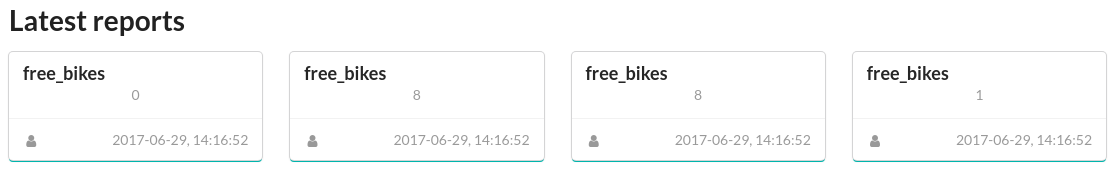
\includegraphics[width=\textwidth]{figuras/latest-reports.png}
    \caption{Página de visualização de resultados.}
  \label{fig:reports}
\end{figure}

O Forensic tem como principais objetivos abstrair o Shock do usuário final,
e consequentemente, as ferramentas de \textit{Big Data} (como o Spark), ao passo em que
fornece um conjunto de funcionalidades que permitem ao usuário final configurar
a atuação dos fluxos, semelhante a outros serviços existentes,
como o Amazon AWS\footnote{\url{https://aws.amazon.com/kinesis/analytics/}}.
Um usuário que deseje interagir com o Shock e o InterSCity deve
(1) configurar um fluxo novo com os
parâmetros desejados; (2) criar esse fluxo no Shock; (3) injetar
esse fluxo no Shock; (4) e iniciar o processamento de fluxos.
O Forensic abstrai esses 4 passos, facilitando o uso
das ferramentas e da plataforma, aproximando usuários finais que não tenham
grande conhecimento do código-fonte do Shock. A Figura \ref{fig:forensicparams}
apresenta a página de visualização e edição de um fluxo, e a Figura
\ref{fig:reports} a página de visualização de resultados processados. Os
resultados de cada dado são mostrados separadamente, onde o título representa
a capacidade do recurso, e o texto centralizado o valor da respectiva capacidade.

Com o propósito de aproximar as soluções que desenvolvemos aos cenários mais
reais, separamos dois casos de uso para serem resolvidos com uso do Forensic e do
Shock. Em cada um desses casos ocorre uma interação entre o InterSCity, Shock e
Forensic, utilizando como produtor de dados alguns coletores de São
Paulo\footnote{\url{https://github.com/lucaskanashiro/collect_sp_data}}. De
maneira geral, os casos de uso abrangem os conceitos citados anteriormente,
como o \textit{cast} de dados, filtros, dentre outros.

\section{CASO DE USO 1 - REGIÕES COM QUALIDADE DO AR INSATISFATÓRIA}

O primeiro caso que separamos é o de regiões que apresentam qualidade do ar
insatisfatória, utilizando como base os dados da
CETESB\footnote{\url{http://sistemasinter.cetesb.sp.gov.br/Ar/php/ar_resumo_hora.php}}
(Companhia Ambiental do Estado de São Paulo).
A solução desse caso de uso pode ser divida em três etapas:
\begin{enumerate}
    \item Coletar os dados;
    \item Publicar os dados no InterSCity;
    \item Configurar um fluxo que filtre os dados, removendo
        da lista os dados com boa qualidade do ar (pois queremos as regiões
        com qualidade insatisfatória).
\end{enumerate}

O primeiro passo, de coleta dos dados, pode ser resolvido via \textit{crawler},
para extrair e normalizar os dados coletados. Um \textit{script} que
utiliza o Mechanize já havia sido desenvolvido por contribuidores do
InterSCity\footnote{\url{https://github.com/lucaskanashiro/collect_sp_data/blob/master/air_quality.rb}},
e pôde ser reaproveitado.

O segundo passo, de publicação dos dados no InterSCity, se baseia na
normalização dos dados e das requisições, para que aja uma interação com o
Resource Adaptor. Adaptamos o \textit{script} mencionado no passo anterior
para que passasse a fazer requisições REST ao Resource Adaptor do InterSCity,
possibilitando o registro de recursos e o envio dos dados.

\lstinputlisting[label={lst:flush1},language=elixir,caption={Consumo dos dados via \textit{websocket}
caso o evento seja \textit{new\_report}.}]{editaveis/arquivos/channel.ex}

O terceiro passo, de configuração do fluxo, é feito através do Forensic.
Um fluxo deve ser criado na interface, e configurado para uso dos
estágios \textit{Kafka Ingestion}, \textit{Kafka Cast} e \textit{Filter}.
O estágio de publicação é mais flexível, e qualquer
estratégia disponível no Forensic serve para esse caso de uso. O Forensic
apresenta uma página de alertas, que é populada via um \textit{flush}
específico apresentado na Listagem \ref{lst:flush1}. Quando esse
\textit{flush} é acionado, o Shock organiza um \textit{job}
que lê de um repositório específico no formato Parquet, e publica no Forensic
via \textit{websocket}.

\begin{figure}[hbt]
  \centering
  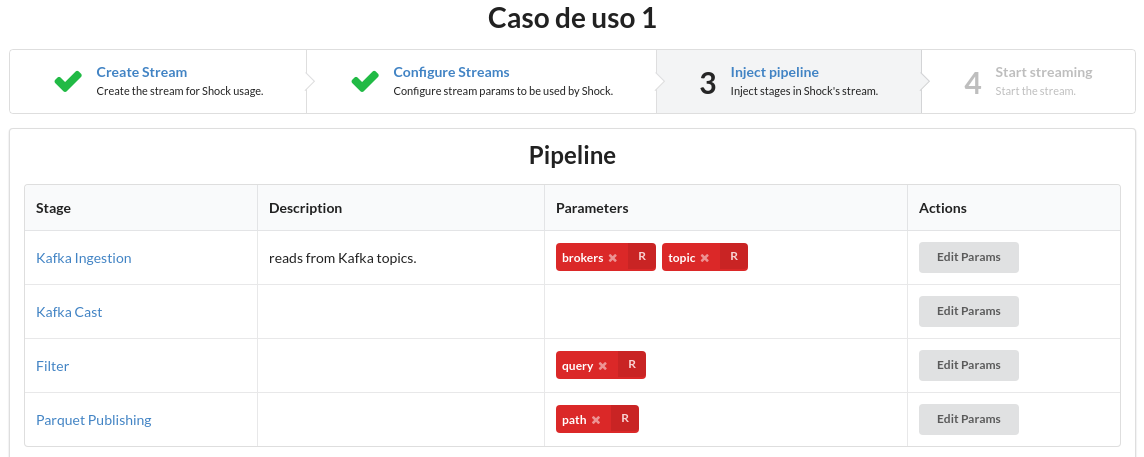
\includegraphics[width=\textwidth]{figuras/parametros.png}
  \caption{Parâmetros do primeiro caso.}
  \label{fig:case1}
\end{figure}

\begin{table}[hbt]
    \centering
    \caption{Parâmetros do fluxo utilizado no primeiro caso de uso.}
    \label{tab:case1}
    \begin{tabular}{|c|c|c|}
        \hline
        \textit{\textbf{Estágio}}                   & \textbf{Parâmetro} & \textbf{Valor}                                         \\ \hline
        \multirow{2}{*}{\textit{Kafka Ingestion}} & \textit{topic}     & \textit{interscity}                                    \\ \cline{2-3} 
                                                  & \textit{brokers}   & \textit{kafka:9092}                                    \\ \hline
                                                  \textit{Kafka Cast}                       & -                  & -                                                      \\ \hline
                                                  \textit{Filter}                           & \textit{query}     & \textit{capability == air\_quality AND value != `boa`} \\ \hline
                                                  \textit{Parquet Publishing}               & \textit{path}      & \textit{/analysis}                                     \\ \hline
    \end{tabular}
\end{table}

Após o fluxo ser criado e os estágios selecionados, basta
configurar os parâmetros e transferir as definições para o Shock. A Figura
\ref{fig:case1} apresenta uma tela do Forensic com o fluxo já
configurado, utilizando os valores presentes na Tabela \ref{tab:case1}.

Por fim, basta seguir os passos de transferência que o Forensic sugere (\textit{Create
Stream, Configure Stream, Inject Pipeline e Start Streaming}), presentes no
topo da Figura \ref{fig:case1}. O Shock então começará o processamento dos
dados, e a próxima vez que o usuário visitar a página de alertas e requisitar
atualização, aparecerão os dados insatisfatórios da qualidade do ar da cidade
de São Paulo.

\section{CASO DE USO 2 - MÉDIA DE BICICLETAS LIVRES NA REGIÃO COM COMBINAÇÃO DE
FLUXOS}

O segundo caso que separamos visa calcular a média de bicicletas livres em estações
de bicicletas de São Paulo, utilizando como base os dados do
CityBik\footnote{\url{https://citybik.es/}}. Esse caso pode ser visto como uma
versão mais complexa do caso anterior, pois deve ser feito o filtro de
capacidades de bicicletas e o cálculo da média dos valores. Ainda,
como mencionado, o Shock só disponibiliza 4 estágios por
fluxos, e como esses requisitos carecem ao menos 5, devem ser criados
dois fluxos, onde o primeiro deve ingerir dados do InterSCity, e o
segundo deve ingerir os resultados do primeiro.

Utilizando os mesmos passos definidos no caso de uso anterior, para o Passo 1
desenvolvemos um
\textit{script}\footnote{\url{https://github.com/lucaskanashiro/collect_sp_data/blob/interscity_integration/citybik.rb}}
que requisita dados à API do CityBik, via REST. Após a ingestão desses dados,
para o Passo 2, o \textit{script} se comunica com o Resource Adaptor,
publicando os dados no InterSCity.

\begin{table}[hbt]
    \centering
    \caption{Parâmetros do primeiro fluxo.}
    \label{tab:case2-1}
    \begin{tabular}{|c|c|c|}
        \hline
        \textit{\textbf{Estágio}}                   & \textbf{Parâmetro} & \textbf{Valor}                      \\ \hline
        \multirow{2}{*}{\textit{Kafka Ingestion}} & \textit{topic}     & \textit{interscity}                 \\ \cline{2-3} 
                                                  & \textit{brokers}   & \textit{kafka:9092}                 \\ \hline
                                                  \textit{Kafka Cast}                       & -                  & -                                   \\ \hline
                                                  \textit{Filter}                           & \textit{query}     & \textit{capability == free\_bikes}  \\ \hline
                                                  \textit{Parquet Publishing}               & \textit{path}      & \textit{/interscity-data/freebikes} \\ \hline
    \end{tabular}
\end{table}

\begin{table}[hbt]
\centering
    \caption{Parâmetros do segundo fluxo.}
\label{tab:case2-2}
\begin{tabular}{|c|c|c|}
\hline
\textit{\textbf{Estágio}}    & \textbf{Parâmetro} & \textbf{Valor}                      \\ \hline
\textit{Parquet Ingestion} & \textit{path}      & \textit{/interscity-data/freebikes} \\ \hline
\textit{Mean}              & -                  & -                                   \\ \hline
\textit{Memory Publishing} & \textit{table}     & \textit{avg}                        \\ \hline
\end{tabular}
\end{table}

Para o Passo 3, devem ser configurados dois fluxos. O primeiro deve
conter os estágios \textit{Kafka Ingestion}, \textit{Kafka Cast},
\textit{Filter} e \textit{Parquet Publishing}, de modo a ingerir novos dados
do InterSCity, filtrar dados não desejados e disponibilizar os dados em formato
Parquet. O segundo fluxo deve conter os estágios
\textit{InterSCity Parquet Ingestion}, \textit{Mean} e alguma forma de
publicação. A ligação entre os dois fluxos ocorre quando o primeiro
publica resultados em um arquivo Parquet, e o segundo
ingere esses resultados como entrada. O valor dos parâmetros
utilizados no primeiro fluxo estão apresentados na Tabela
\ref{tab:case2-1}, e os parâmetros do segundo fluxo na Tabela
\ref{tab:case2-2}. Após a configuração dos parâmetros e transferência das
configurações para o Shock, semelhante ao ocorrido no caso de uso anterior,
os dois fluxos começam o processamento dos dados, retornando para o
Forensic a média de bicicletas disponíveis na região.
